\chapter{Fermions, Dirac Matrices, and the Dirac Sea}

This lecture begins with a promise and an interruption. Leonard Susskind opens by invoking the Dirac sea, but before going there he deliberately backs up: first to the difference between bosons and fermions in second quantization, then to the simpler one-dimensional Dirac construction, and only then to the three-dimensional equation appropriate to the physical world. That order matters. The later discussion of holes and positrons depends on the earlier algebra of fermions, and the later \(4\times 4\) Dirac matrices are introduced only after the \(2\times 2\) theory has been pushed until it fails. These notes follow that progression closely. Throughout, we normalize the lecture's shifting notation by writing operator equations with \(P\) or \(\mathbf P\), and eigenvalue relations with \(p\) or \(\mathbf p\). We use units \(c=\hbar=1\).

\section{Fermionic Exchange and Anti-Commutation}

Before returning to the Dirac equation, Susskind asks how many-particle systems are built from field operators, and in particular how fermions differ from bosons. The first point is familiar but important: bosons may occupy the same state, while fermions may not. He wants that statement to arise from operator algebra.

Take a two-particle state created from the vacuum,
\begin{equation}
|x,y\rangle=\psi^\dagger(x)\psi^\dagger(y)|0\rangle.
\end{equation}
Here \(x\) and \(y\) label the positions of particle \(1\) and particle \(2\); they are not the \(x\)- and \(y\)-coordinates of one particle. For bosons, exchanging the two particles changes nothing:
\begin{equation}
|x,y\rangle=|y,x\rangle.
\end{equation}
At the operator level this is implemented by commuting creation operators,
\begin{equation}
\psi^\dagger(x)\psi^\dagger(y)=\psi^\dagger(y)\psi^\dagger(x).
\end{equation}

For fermions the exchanged state picks up a minus sign,
\begin{equation}
|x,y\rangle=-|y,x\rangle.
\end{equation}
An overall sign of a state vector is not itself observable, but the sign is crucial in the formulas, and Susskind's point is that the formulas force the field operators to anti-commute. The transcript-backed completion of the partially obscured board equation is
\begin{equation}
\psi^\dagger(x)\psi^\dagger(y)=-\,\psi^\dagger(y)\psi^\dagger(x).
\end{equation}

\begin{definition}
For two operators \(A\) and \(B\), the anti-commutator is
\begin{equation}
\{A,B\}=AB+BA.
\end{equation}
\end{definition}

So the fermionic relation is equivalently
\begin{equation}
\{\psi^\dagger(x),\psi^\dagger(y)\}=0.
\end{equation}
This is the lecture's first decisive step: exchange antisymmetry is translated into the algebra of creation operators.

\begin{figure}
\centering

\includegraphics[width=0.76\textwidth]{lecture_10_figure_02.png}
\caption{Fermionic minus-sign operator step from exchange antisymmetry. The right-hand side is partly hidden on the board, so the notes use the transcript-backed completion \(\psi^\dagger(x)\psi^\dagger(y)=-\,\psi^\dagger(y)\psi^\dagger(x)\).}
\end{figure}

Susskind then immediately specializes to the case \(y=x\). This is the lecture's route to the exclusion principle. Starting from the anti-commutator,
\begin{align}
\{\psi^\dagger(x),\psi^\dagger(x)\}=0
&\Longrightarrow \psi^\dagger(x)\psi^\dagger(x)+\psi^\dagger(x)\psi^\dagger(x)=0 \\
&\Longrightarrow 2\,\psi^\dagger(x)\psi^\dagger(x)=0 \\
&\Longrightarrow (\psi^\dagger(x))^2=0.
\end{align}
Trying to create two identical fermions in the same state gives the zero vector, not a new state.

\begin{figure}
\centering

\includegraphics[width=0.80\textwidth]{lecture_10_figure_03.png}
\caption{Equal-point anti-commutator and exclusion-principle simplification. The visible board equation already shows the factor \(2\), the repeated creation-operator product at \(x\), and the vanishing result.}
\end{figure}

Because the board is visually important here, it is worth pairing it with a clean reconstruction of the logical chain:

\begin{figure}
\centering
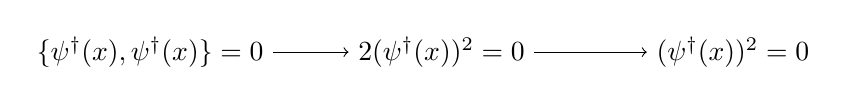
\begin{tikzpicture}[node distance=3.7cm]
\node (a) {$\{\psi^\dagger(x),\psi^\dagger(x)\}=0$};
\node (b) [right of=a] {$2(\psi^\dagger(x))^2=0$};
\node (c) [right of=b] {$(\psi^\dagger(x))^2=0$};
\draw[->] (a) -- (b);
\draw[->] (b) -- (c);
\end{tikzpicture}
\caption{Clean reconstruction of the equal-point fermionic exclusion step.}
\end{figure}

\section{Occupation Numbers and the Filled/Empty Symmetry}

Susskind does not move on as soon as exclusion has been obtained. He lingers on the algebra long enough to extract a second idea, one that he explicitly says will matter later: for a single fermionic mode, creation and annihilation operators are algebraically more symmetric than for bosons.

For a single bosonic mode one may summarize the usual structure by
\begin{equation}
[a,a^\dagger]=1,
\qquad
n_{\text{boson}}=0,1,2,\dots
\end{equation}
The occupation-number ladder stretches upward without bound. The annihilation operator eventually reaches the bottom and gives zero; the creation operator never runs out of states above it. In that very concrete sense the bosonic ladder distinguishes ``up'' from ``down.''

For a single fermionic mode the algebra is instead
\begin{equation}
\{a,a^\dagger\}=1,
\qquad
a^2=(a^\dagger)^2=0,
\qquad
n_{\text{fermion}}=0,1.
\end{equation}
There are only two possibilities: empty or filled. The creation operator takes \(0\) to \(1\), but acting once more gives zero because there is no state above \(1\). The annihilation operator takes \(1\) to \(0\), but acting once more gives zero because there is no state below \(0\).

So the single-mode fermionic spectrum is symmetric in a way the bosonic spectrum is not. Empty and filled exchange roles under \(a\leftrightarrow a^\dagger\). Physically the two operators still do different things, but algebraically one cannot tell them apart as sharply as in the bosonic case. Susskind pauses here to emphasize that this is not yet a claim about particles and anti-particles; it is simply a structural fact about fermionic operators. But it is exactly the fact that later makes the hole interpretation feel natural rather than miraculous.

\begin{remark}
In the lecture Susskind comes back to this point much later, when the annihilation of a negative-energy electron is reinterpreted as the creation of a positron. The symmetry between filled and empty states is prepared here, not inserted retroactively at the end.
\end{remark}

\section{Review of the One-Dimensional Dirac Construction}

Having put the fermionic operator algebra in place, Susskind says, in effect, let us go back to the Dirac equation. For the moment he again works at the single-particle level.

The starting point is the one-dimensional massless equation
\begin{equation}
i\partial_t\psi=-\,i\partial_x\psi.
\end{equation}
This is a Schr\"odinger equation with Hamiltonian
\begin{equation}
H=P,
\end{equation}
so on momentum eigenstates
\begin{equation}
E=p.
\end{equation}
Wave packets move rigidly to the right. It is a perfectly good relativistic equation for a massless right-mover, but it is not yet a satisfactory model of a massive electron.

The relativistic target is
\begin{equation}
E^2=p^2+m^2.
\end{equation}
Before adding mass, however, Susskind first doubles the one-dimensional theory by introducing a left-moving partner:
\begin{equation}
H\psi_1=P\psi_1,
\qquad
H\psi_2=-P\psi_2.
\end{equation}
Now one has two species, one always moving to the right and one always moving to the left. Packaging them into a two-component wavefunction,
\begin{equation}
\psi=
\begin{pmatrix}
\psi_1\\
\psi_2
\end{pmatrix},
\end{equation}
one introduces a matrix \(\alpha\) with eigenvalues \(+1\) and \(-1\),
\begin{equation}
\alpha=
\begin{pmatrix}
1&0\\
0&-1
\end{pmatrix},
\end{equation}
so that both equations are summarized by
\begin{equation}
H\psi=\alpha P\,\psi.
\end{equation}
This doubles the number of components and introduces an internal two-valued degree of freedom. In the one-dimensional lecture review Susskind interprets it as handedness: right-moving versus left-moving.

Mass still has not appeared. To generate it, he introduces a second matrix \(\beta\) which couples the two sectors. In the one-dimensional construction the convenient choice is
\begin{equation}
\beta=
\begin{pmatrix}
0&1\\
1&0
\end{pmatrix},
\end{equation}
and one writes
\begin{equation}
H=\alpha P+\beta m.
\end{equation}
The required algebra is
\begin{equation}
\alpha^2=1,
\qquad
\beta^2=1,
\qquad
\alpha\beta+\beta\alpha=0.
\end{equation}
Susskind explicitly warns that this is matrix anti-commutation, not the anti-commutation of fermionic fields.

Now the worked derivation is straightforward:
\begin{align}
H^2
&=(\alpha P+\beta m)^2 \\
&=\alpha^2P^2+\alpha\beta Pm+\beta\alpha mP+\beta^2m^2 \\
&=\alpha^2P^2+(\alpha\beta+\beta\alpha)Pm+\beta^2m^2 \\
&=P^2+m^2.
\end{align}
Thus the mass term works because the cross term cancels. Susskind's physical gloss is that the off-diagonal matrix couples left-moving and right-moving sectors. He immediately qualifies the picture, but the picture is still useful: mass behaves like a term that mixes the two handed motions, and that is why a massive particle can be thought of as capable, in some averaged sense, of being at rest.

\section{From One Dimension to Three: \texorpdfstring{$H=\boldsymbol{\alpha}\cdot\mathbf P$}{H=alpha.P}}

The lecture's next hard pivot is explicit: how do we do this in three dimensions?

The one-dimensional Hamiltonian \(H=\alpha P\) cannot simply be copied, because now momentum is a three-vector. The board writes
\begin{equation}
H=\alpha\cdot P,
\end{equation}
and Susskind's point is that \(\alpha\) must therefore become a vector of matrices. In normalized notation we write the operator equation as
\begin{equation}
H=\boldsymbol{\alpha}\cdot\mathbf P
=\alpha_xP_x+\alpha_yP_y+\alpha_zP_z.
\end{equation}

\begin{figure}
\centering

\includegraphics[width=0.82\textwidth]{lecture_10_figure_04.png}
\caption{Three-dimensional Dirac ansatz \(H=\boldsymbol{\alpha}\cdot\mathbf p\). The board writes \(H=\alpha\cdot P\); the notes normalize this to the operator form \(H=\boldsymbol{\alpha}\cdot\mathbf P\).}
\end{figure}

For a massless relativistic particle the desired dispersion relation is
\begin{equation}
E^2=\mathbf p^2=p_x^2+p_y^2+p_z^2.
\end{equation}
Accordingly one wants the operator identity
\begin{equation}
H^2=\mathbf P^2.
\end{equation}
Squaring the Hamiltonian gives
\begin{align}
H^2
&=\alpha_x^2P_x^2+\alpha_y^2P_y^2+\alpha_z^2P_z^2 \\
&\quad+(\alpha_x\alpha_y+\alpha_y\alpha_x)P_xP_y \\
&\quad+(\alpha_x\alpha_z+\alpha_z\alpha_x)P_xP_z \\
&\quad+(\alpha_y\alpha_z+\alpha_z\alpha_y)P_yP_z.
\end{align}
Thus the matrices must satisfy
\begin{equation}
\alpha_x^2=\alpha_y^2=\alpha_z^2=1,
\qquad
\alpha_i\alpha_j+\alpha_j\alpha_i=0
\quad (i\neq j).
\end{equation}
The cross terms vanish only if the different \(\alpha_i\) mutually anti-commute.

Here the lecture arrives at the Pauli matrices. They satisfy exactly the required algebra:
\begin{equation}
\sigma_x=
\begin{pmatrix}
0&1\\
1&0
\end{pmatrix},
\qquad
\sigma_y=
\begin{pmatrix}
0&-i\\
i&0
\end{pmatrix},
\qquad
\sigma_z=
\begin{pmatrix}
1&0\\
0&-1
\end{pmatrix}.
\end{equation}
So one may take
\begin{equation}
\alpha_x=\sigma_x,
\qquad
\alpha_y=\sigma_y,
\qquad
\alpha_z=\sigma_z.
\end{equation}
The Hamiltonian then becomes
\begin{equation}
H=\boldsymbol{\sigma}\cdot\mathbf P.
\end{equation}

\begin{figure}
\centering

\includegraphics[width=0.76\textwidth]{lecture_10_figure_05.png}
\caption{Massless Hamiltonian summarized as \(H=\boldsymbol{\sigma}\cdot\mathbf p\). The board's compact formula follows the explicit component-by-component identification of the three \(\alpha_i\) with the Pauli matrices.}
\end{figure}

A clean way to state the resulting spectrum is
\begin{equation}
\boldsymbol{\sigma}\cdot\mathbf p
=
|\mathbf p|\,(\boldsymbol{\sigma}\cdot\hat{\mathbf p}),
\qquad
\hat{\mathbf p}=\frac{\mathbf p}{|\mathbf p|}.
\end{equation}
Since \(\boldsymbol{\sigma}\cdot\hat{\mathbf p}\) has eigenvalues \(\pm1\), the energy eigenvalues are
\begin{equation}
E=\pm |\mathbf p|.
\end{equation}
This is the mathematically clean form of Susskind's explanation that the energy is the component of spin along the momentum direction. Positive energy corresponds to spin aligned with momentum; negative energy corresponds to spin anti-aligned with momentum.

\begin{remark}
The transcript is corrupted at the point where Susskind responds to the claim that spin somehow ``drops out'' of the Dirac equation. The surrounding logic is nevertheless clear. Dirac wanted a Hamiltonian linear in momentum; ordinary numbers could not do the job; the Pauli matrices were forced on him by the requirement \(H^2=\mathbf P^2\). In that sense spin is not tacked on afterward but emerges from the linearization logic itself.
\end{remark}

\section{Why Mass Forces \texorpdfstring{$4\times4$}{4x4} Matrices}

At this stage Susskind immediately asks the next question: if the \(2\times2\) massless theory works so neatly, why not just add a mass term to it? The natural trial is
\begin{equation}
H=\boldsymbol{\sigma}\cdot\mathbf P+\beta m.
\end{equation}
Assuming again that \(\beta^2=1\), squaring \(H\) would give the desired \(m^2\) term, but only if the cross term vanishes. That requires
\begin{equation}
\sigma_i\beta+\beta\sigma_i=0
\qquad
(i=x,y,z).
\end{equation}
So \(\beta\) would have to anti-commute with all three Pauli matrices.

That is precisely what fails. In \(2\times2\) matrices the Pauli matrices already exhaust the family of mutually anti-commuting matrices. There is no further \(2\times2\) matrix that anti-commutes with all three. This is the lecture's algebraic obstruction: the three-dimensional \(2\times2\) equation is intrinsically massless.

The next step is therefore not a matter of taste. One must enlarge the internal vector space and look for \(4\times4\) matrices. Susskind emphasizes that the first matrix size supporting four mutually anti-commuting matrices is \(4\times4\), and that this is a mathematical fact about matrix algebras, not a consequence of spacetime having four dimensions.

A convenient representation, consistent with the block description given in the lecture, is
\begin{equation}
\alpha_i=
\begin{pmatrix}
\sigma_i&0\\
0&-\sigma_i
\end{pmatrix},
\qquad
\beta=
\begin{pmatrix}
0&I\\
I&0
\end{pmatrix}.
\end{equation}
These satisfy
\begin{equation}
\{\alpha_i,\alpha_j\}=2\delta_{ij},
\qquad
\{\alpha_i,\beta\}=0,
\qquad
\beta^2=1.
\end{equation}
The Hamiltonian becomes
\begin{equation}
H=\boldsymbol{\alpha}\cdot\mathbf P+\beta m,
\end{equation}
or explicitly
\begin{equation}
H=
\begin{pmatrix}
\boldsymbol{\sigma}\cdot\mathbf P & mI\\
mI & -\boldsymbol{\sigma}\cdot\mathbf P
\end{pmatrix}.
\end{equation}
Its square is then
\begin{equation}
H^2=\mathbf P^2+m^2.
\end{equation}

\begin{remark}
The lecture moves quickly through the explicit matrices and repeatedly reminds the audience that many equivalent representations exist. The representation above should therefore be read as a cautious standard reconstruction matching Susskind's block-wise description, not as a uniquely privileged choice.
\end{remark}

What matters is the structure: the massive three-dimensional Dirac equation needs a four-component spinor because the \(2\times2\) matrix algebra is too small to accommodate the extra anti-commuting matrix required by the mass term.

\section{Chirality, Velocity, and Spin}

Once the \(4\times4\) theory is on the board, the lecture turns to interpretation. Several student questions now become part of the mathematical story.

\paragraph{Chirality and the mass term.}
In the massless \(2\times2\) theory, positive energy ties the spin to the momentum. In the lecture Susskind speaks of chirality as the relation between the two, so that one alignment is right-handed and the opposite alignment is left-handed. In more standard language, for the massless case this is the same idea that is often called helicity.

The crucial point is that the \(2\times2\) massless theory contains only one handedness at a time. The \(4\times4\) enlargement brings in the opposite handedness as well, and the off-diagonal \(\beta m\) term mixes the two blocks. That is why Susskind repeatedly describes the mass term as a coupling between left-handed and right-handed sectors. For a massless particle the handedness is conserved; with the mass term present, transitions between the two become possible.

\paragraph{Velocity from the Heisenberg equation.}
Susskind then asks a more surprising question: what physical observable is represented by the matrices \(\alpha_i\)? His answer is that \(\alpha_i\) are the components of the velocity operator.

Using the Heisenberg equation in the standard form
\begin{equation}
\dot L=i[H,L],
\end{equation}
together with the canonical commutator
\begin{equation}
[x,P_x]=i,
\end{equation}
we compute
\begin{align}
\dot x
&=i[H,x] \\
&=i[\alpha_xP_x+\alpha_yP_y+\alpha_zP_z+\beta m,\;x] \\
&=i\alpha_x[P_x,x] \\
&=\alpha_x.
\end{align}
The matrices commute with \(x\) because they act in the internal spinor space, not in position space. So only \(P_x\) contributes. The conclusion is the lecture's punchline:
\begin{equation}
\dot x=\alpha_x.
\end{equation}

\begin{remark}
Susskind explicitly says that he does not remember the sign convention in the Heisenberg equation and does not care to stop and fix it. The convention used here is the standard one. The only indispensable lecture claim is the resulting identification \(\dot x=\alpha_x\).
\end{remark}

Each \(\alpha_i\) has eigenvalues \(\pm1\), so an instantaneous measurement of a velocity component yields \(\pm1\) in our units. But that is not the end of the story, because the velocity operator is not conserved:
\begin{equation}
\dot\alpha_x=i[H,\alpha_x]\neq0.
\end{equation}
The Hamiltonian contains \(\alpha_y\) and \(\alpha_z\), and they do not commute with \(\alpha_x\). Hence the velocity oscillates. This is Susskind's discussion of \emph{zitterbewegung}: the rapid trembling motion of the free Dirac electron.

He is careful to separate this from the conservation of momentum. Newton's law says that the momentum of a free particle is constant; it does not say that every operator one might call ``velocity'' must be constant. In this theory momentum and velocity are not the same operator. The lecture keeps the explanation qualitative, but the basic point is that the time average of the rapidly fluctuating velocity reproduces the expected smooth motion, and for slow particles that average velocity is \(P/m\).

\paragraph{Velocity is not spin.}
A further student question prompts an important clarification. The matrices \(\alpha_i\) are not the genuine spin operators. They transform as an ordinary vector; spin is an axial vector. In the block notation above, a natural corresponding spin operator is
\begin{equation}
\Sigma_i=
\begin{pmatrix}
\sigma_i&0\\
0&\sigma_i
\end{pmatrix},
\end{equation}
which differs from \(\alpha_i\) by the sign in the lower block. Susskind's point is that the Dirac electron carries more internal structure than a single naive ``spin'' label. One binary distinction is tied to handedness; another is the actual spin of the electron.

The lecture briefly detours through quaternions because a student asks about them. The only lasting point for us is that the Pauli matrices sit inside a very rigid algebraic structure. The quaternion aside itself is not part of the main mathematical spine, and Susskind does not use it in what follows.

\section{Negative Energy, the Dirac Sea, and Positrons}

Only now does the lecture finally return to its announced destination. Susskind immediately simplifies the setting again. To discuss negative energy one does not need the full \(3+1\)-dimensional Dirac equation; the essential issue is already present in the simplest one-dimensional right-moving massless case,
\begin{equation}
H=P.
\end{equation}
Because \(P\) can take either sign, the theory contains both positive- and negative-energy states.

This is dangerous. The vacuum should be the state of lowest energy. If one can keep adding negative-energy particles, then the energy can be driven downward without bound and there is no stable vacuum. Susskind's resolution is historical and explicitly Diracian: since the particles are fermions, every negative-energy state can be occupied at most once. Therefore the lowest-energy state is obtained by filling all negative-energy states. That filled configuration is the Dirac sea.

The lecture stresses that if the particles were bosons this would fail. One could put arbitrarily many bosons into the same negative-energy state and the energy would continue to decrease. So the stability of the Dirac vacuum depends crucially on Fermi statistics.

Once the negative-energy states are filled, two kinds of excitations remain. One may add an ordinary positive-energy electron above the sea. Or one may remove a negative-energy electron from the sea. The removed electron leaves a hole. Since the missing object carried negative charge, the hole carries positive charge. Since removing a negative-energy particle raises the energy, the hole has positive energy:
\begin{equation}
E_{\text{hole}}=-E_{\text{negative electron}}>0.
\end{equation}
That hole is the positron.

At this point the lecture returns to the earlier algebraic symmetry of fermionic operators. The field operator is first written schematically as an integral over all momenta,
\begin{equation}
\psi(x)\sim \int_{-\infty}^{\infty} dp\, a(p)e^{-ipx}.
\end{equation}
Susskind then splits the integral into positive- and negative-momentum pieces,
\begin{equation}
\psi(x)\sim
\int_{0}^{\infty} dp\, a(p)e^{-ipx}
+
\int_{-\infty}^{0} dp\, a(p)e^{-ipx}.
\end{equation}
The second piece annihilates negative-energy electrons. Using the fermionic symmetry between filled and empty states, one reinterprets that operator as a positron creation operator. Writing schematically
\begin{equation}
b^\dagger(p)\equiv a(-p),
\end{equation}
the field becomes
\begin{equation}
\psi(x)\sim
\int_0^\infty dp\, a(p)e^{-ipx}
+
\int_0^\infty dp\, b^\dagger(p)e^{ipx}.
\end{equation}
The first term annihilates positive-energy electrons; the second creates positrons. The precise normalization and phase conventions are not the point here. The lecture's point is the structural split.

Susskind then inserts this idea into the schematic interaction term
\begin{equation}
H_{\mathrm{int}}\sim \psi^\dagger(x)\psi(x)A(x).
\end{equation}
Because \(\psi\) and \(\psi^\dagger\) each contain both electron and positron pieces, the same operator contains several processes at once. Depending on which pieces are selected, it can describe
\begin{enumerate}
\item an electron emitting or absorbing a photon,
\item an electron and a positron annihilating into a photon,
\item a photon creating an electron-positron pair.
\end{enumerate}
This is Susskind's way of showing that a single field-theoretic coupling encodes many different channels, which later become the lines and vertices of Feynman-diagram language.

The lecture then shifts from Dirac's historical picture to the more modern reinterpretation. Modern physicists usually do not describe the vacuum as literally full of negative-energy electrons. Instead they simply flip the operator assignments in the negative-energy sector from the start. Creation operators for negative-energy electrons are replaced by annihilation operators for positive-energy positrons, and the symmetry between electrons and positrons becomes manifest at once. Susskind nevertheless keeps Dirac's sea in the foreground because it captures the logic of the discovery.

He closes with the condensed-matter analogy. In a crystal, electrons fill states up to the Fermi level; removing one leaves a hole; that hole behaves as a positive charge carrier with positive energy measured relative to the filled ground state. The pattern is strikingly similar: a filled sea, particles above it, and holes within it. The analogy is pedagogically valuable, even though historically Dirac arrived at his picture before the solid-state language became familiar.

Finally, in response to questions, Susskind distinguishes the fermionic Dirac story from the bosonic Klein--Gordon story. The Klein--Gordon equation is structurally different; it is not simply a Hamiltonian linear in momentum with Dirac matrices, and he does not attempt to fold it into the same narrative in this lecture.

\section{Summary}

The lecture unfolds as a chain of necessities rather than a list of topics. Fermionic exchange symmetry leads to anti-commuting creation operators, and the equal-point specialization gives exclusion. The two-state fermionic occupation number then prepares the later particle-hole reinterpretation. Only after that groundwork is in place does Susskind review the one-dimensional Dirac equation, add the left-moving partner, and show that a mass term is a coupling that mixes the two sectors.

From there the move to three dimensions is forced by rotational invariance. The demand that a Hamiltonian be linear in momentum and yet satisfy \(H^2=\mathbf P^2\) produces the Pauli matrices and the massless Hamiltonian \(H=\boldsymbol{\sigma}\cdot\mathbf P\). The failure of any \(2\times2\) mass term then forces the jump to \(4\times4\) Dirac matrices, where mass becomes a coupling between opposite chiralities. The interpretation of \(\alpha\) as velocity, the nonconservation of velocity, and the distinction between \(\alpha\) and true spin are all consequences of that enlarged structure.

Only after those algebraic and kinematical steps are laid down does the original promise return. Negative energy is stabilized by Fermi statistics, the filled Dirac sea becomes the vacuum, holes become positrons, the fermion field splits into electron-annihilation and positron-creation parts, and a simple interaction term already contains emission, annihilation, and pair creation. The lecture thus ends where it began, but with all the necessary machinery now in place.